%!TEX root = main.tex
\section{Introduction}

Computation Application Language (CAL) is designed to write large scale application in due to perform big data processing. Each CAL program consists of modules that are separetely executed in sequence (with parallelization possibility) on virtual machines and sending the results futher to next module of an application. CAL language is a part of the system developed under the Baltic LSC\cite{baltic_lsc_website} project.

During the data processing within the application run, each module is executed with some input data. It could be different kind of data e.g. data frame or set of images. The execution of a module is invoke on a virtual machine with limited resources (RAM, mCPUs, GPUs). The details of an input data and the execution environment resources will be used to estimate the overall application execution time and price on a concrete cluster.

Baltic Large Scale Computing (BalticLSC\cite{baltic_lsc}) project is using CAL language to perform data processing tasks. Each task is an execution of a CAL application. Each module can be used in many CAL applications. We can say that a single module is a one block (commonly as a docker image) and an application is the schema of executing concrete set of blocks. Figure~\ref{fig:example_app} shows the example application that consits of a few modules to perform some image processing. Some of the modules (\textit{R}, \textit{G} and \textit{B} \textit{processors}) can be executed in parallel.

\begin{figure*}[!t]
	\centering
	\begin{minipage}{0.9\linewidth}
	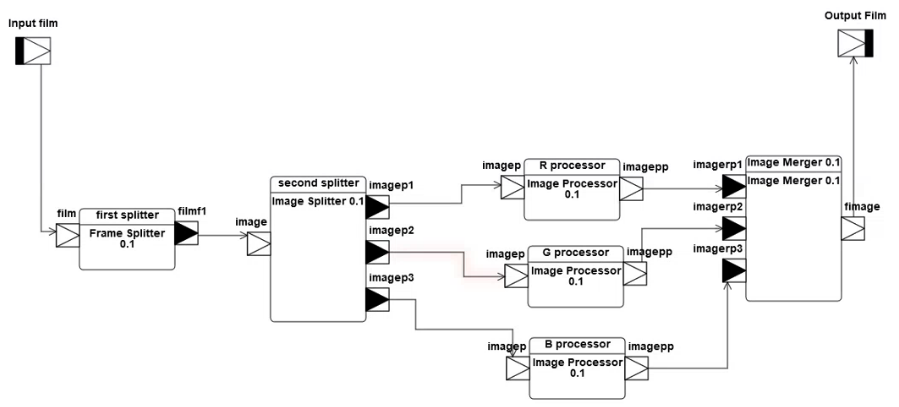
\includegraphics[width=1.0\textwidth]{example_app}
	\end{minipage}
	\caption{The example of an image processing application written in the CAL language.}
	\label{fig:example_app}
\end{figure*}

The aim of this project is to estimate the module execution time based on input data and limited resources of the execution. The choosen approach is to create machine learning models using historical data of the module executions times.

The WCET\footnote{Worst-case execution time - the maximum amout of time that the execution can take.} execution time is a crucial feature of a real-time systems\cite{wcet} when response should be guaranteed within a specified timing constraint or system should meet the specified deadline. In this project we do not strictly focus on providing an estimation of maximum execution time (WCET). We will try to estimate the average-case execution time (ACET) which is absolutely enought for this use case requirements.